\documentclass[../main.tex]{subfiles}
\begin{document}

\subsection{Categorical}

\subsubsection{Cross Tabulation Visualization}
\begin{figure}
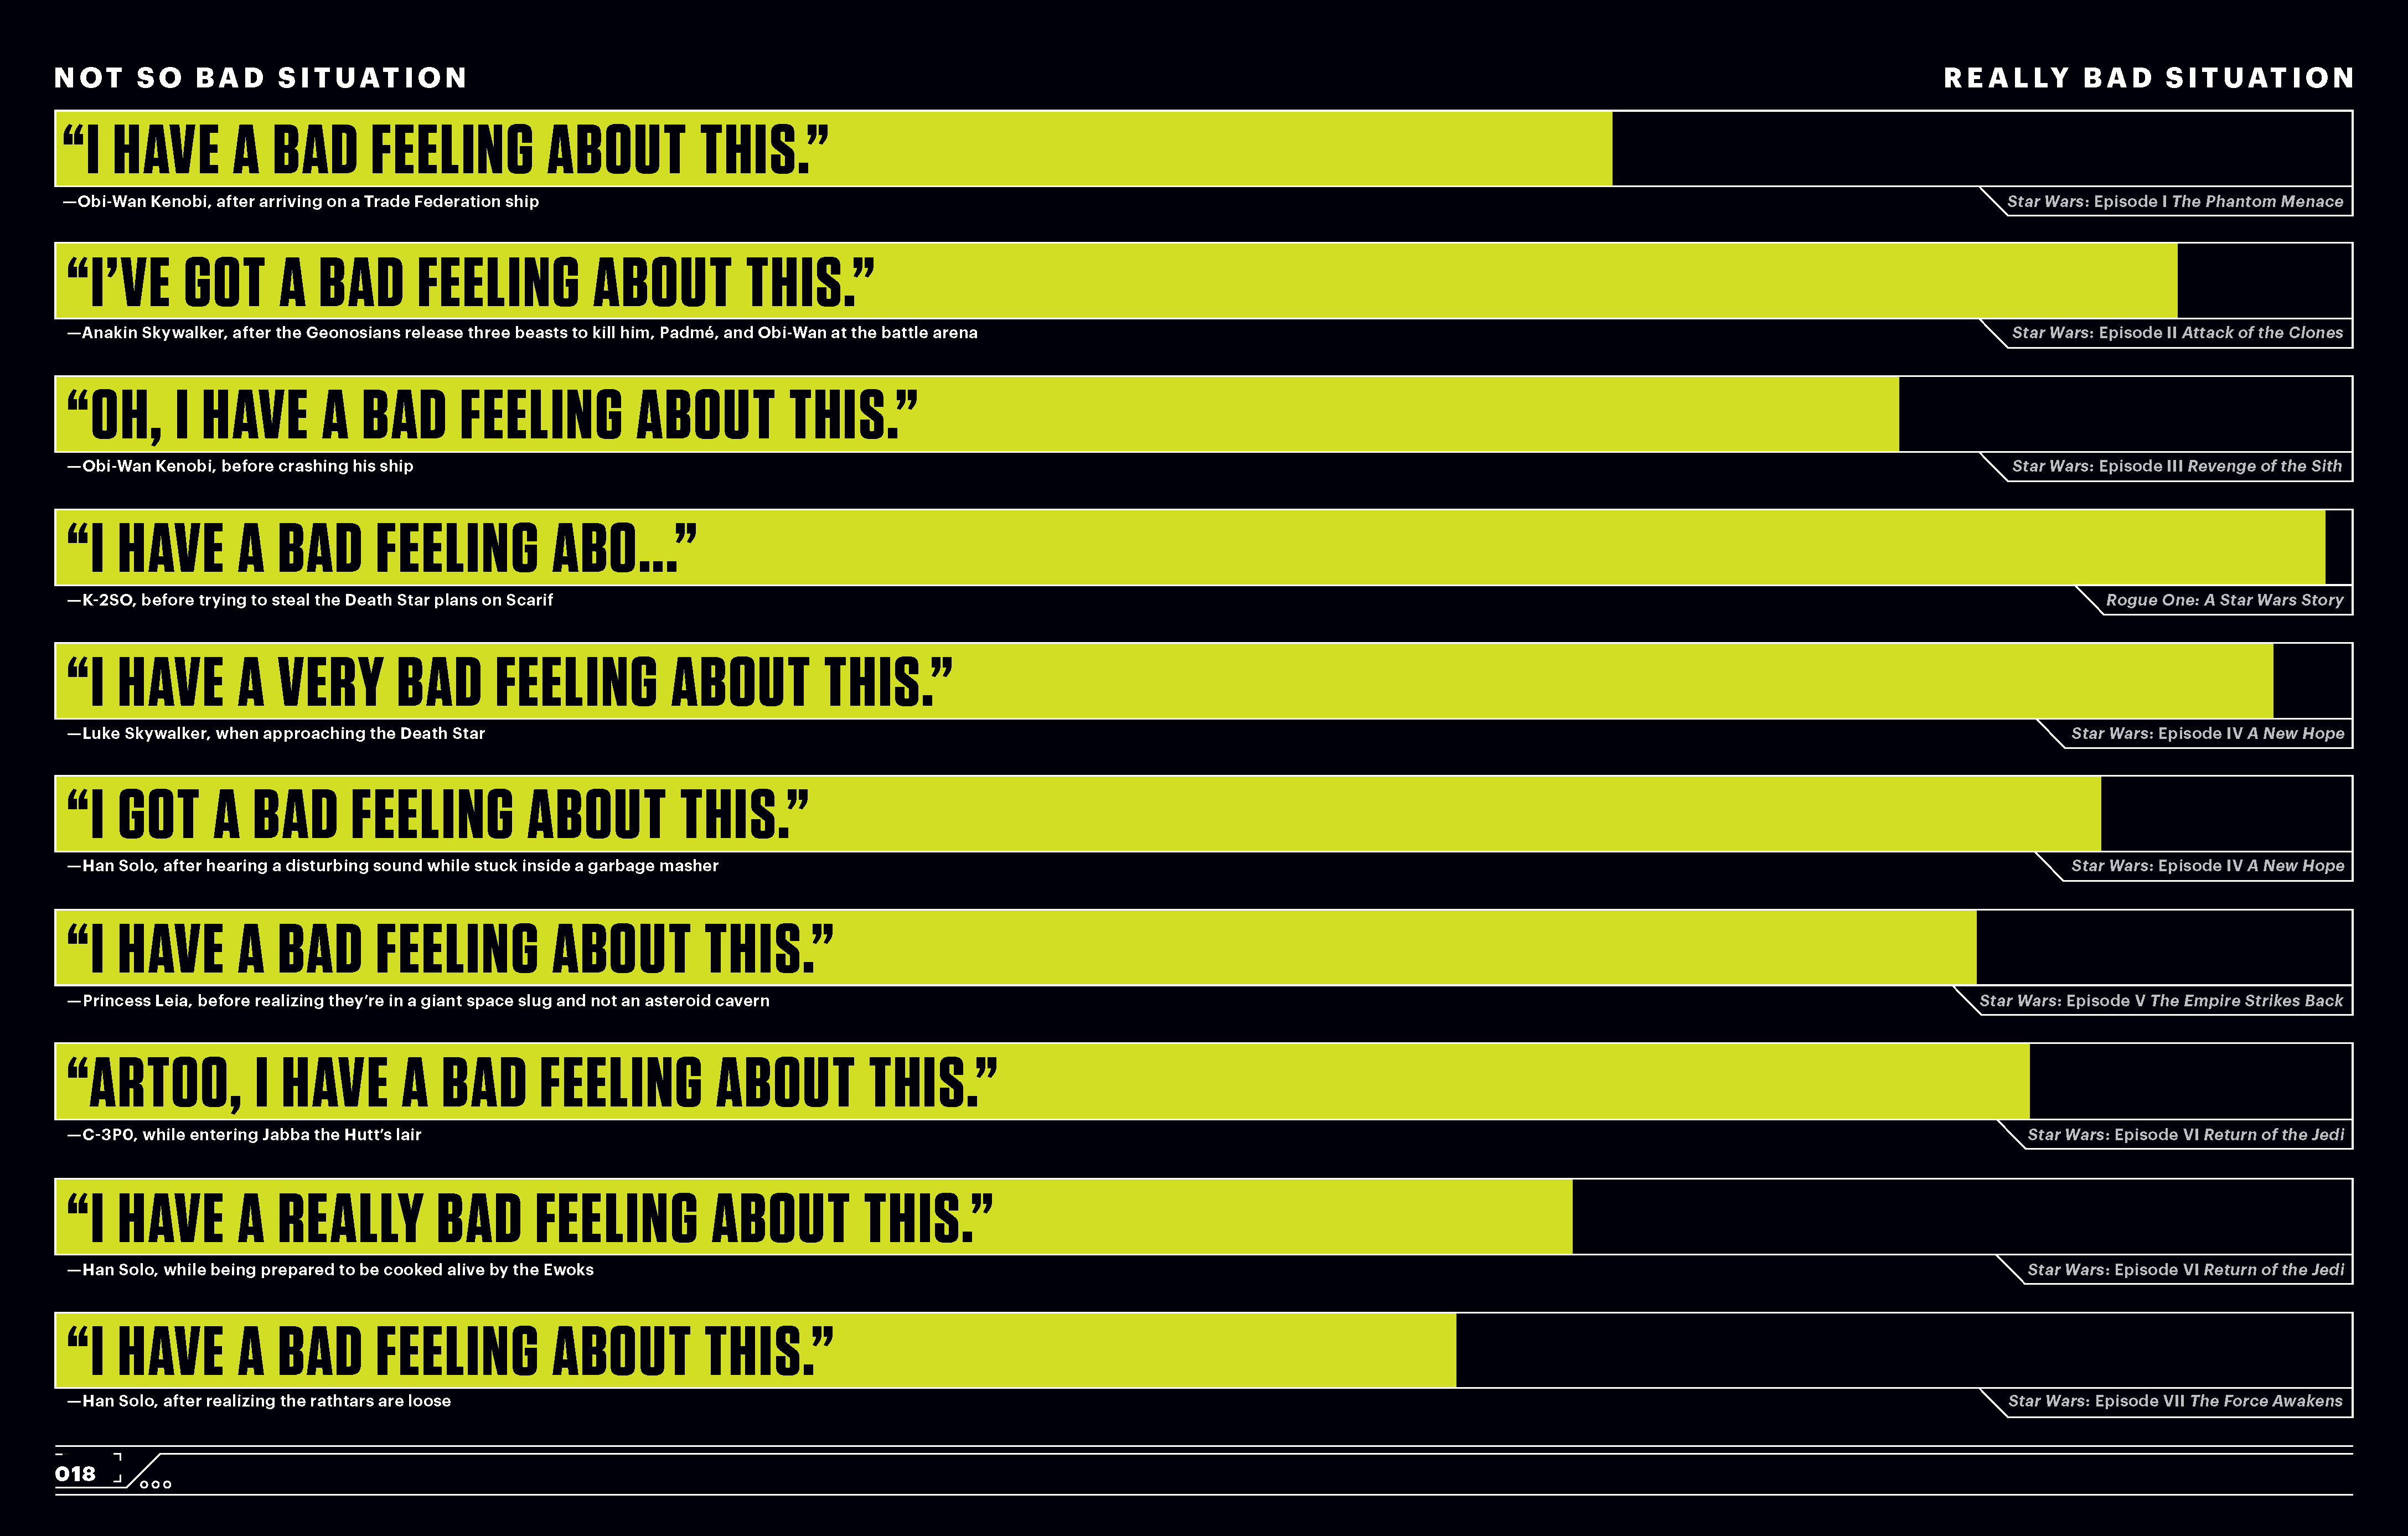
\includegraphics[width=1\textwidth]{swsg.png}
\caption{Graphic designer Tim Leong visualizes a cross tabulation of the severity of a situation against the language used in each situation to show the relative frequency of really bad situations in Star Wars. The ordering of the phrases by the order in which the movies came out and the slight semantic variations between each phrase can be further mined for potential conditional dependencies between these underlying aspects of the phrase, the phrase itself, and the severity of the situation. Chart is from Star Wars Super Graphic \cite{leong_star_2017}}
\label{fig:starwars}
\end{figure}

Categorical data can be likened to set measurement, where each category is a set
and researchers often want to know how many members each set has and what
intersections are common between sets \cite{agresti_categorical_2011,schneider_set-theoretic_2012}. In exploring these intersections, the question arises of which categories appear in conjunction with each other and if any one category is the driving force underlying the other categories. For example in frequent item set detection, the task is explicitly to figure out what is the minimum set of items that can be used to predict the occurrence of other items in the basket \cite{leskovec_mining_2014,Srikant:1997:MAR:3001392.3001404} The most common approach is to create a list of frequencies, sometimes of sets of one category or a cross-table\cite{goodman_measures_1991} which is an aggregate function applied to the product of two or more sets. A visual example of a simple cross tabulation can be see in figure~\ref{fig:starwars}, wherein designer Tim Leong looks at the probability of a situation being bad given the structure and content of a given phrase\cite{leong_star_2017}. Each phrase acts as set of size 1, the cross tabulation in this case being the likelihood of the situation being bad. Because the phrases are ordered in temporal order, Leong's visualization suggests that there's a higher likelihood of bad events happening near the middle of the time-line, indicating that severity of situational badness and the type of phrasing used could be conditionally dependent on the location of the story arc. 

\begin{figure}
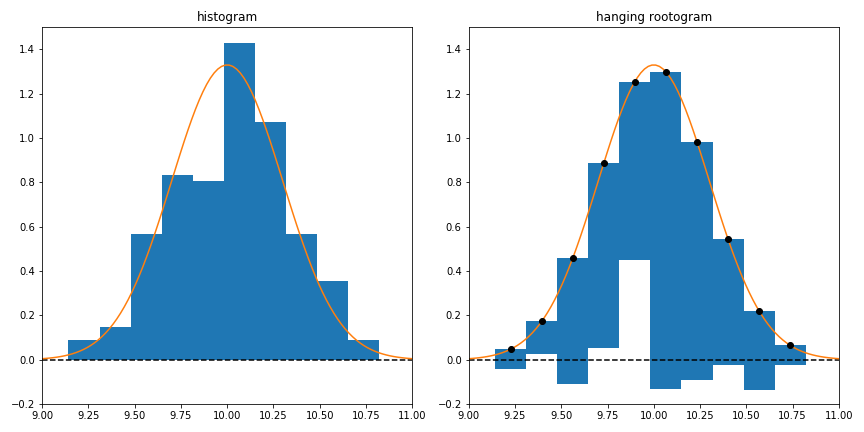
\includegraphics[width=1\textwidth]{hanging_rootgram.png}
\caption{The hanging rootogram moves the histogram bars so that they meet the expected values of the density estimator. This in turn means that deviations between the expected and observed frequencies can be measured more easily as distance between the bottom of the rectangle to a horizontal 0, rather than as a difference between the top of the rectangle and a point on a distribution curve.}
\label{fig:hanging_rootogram}
\end{figure}

 While a table is encouraged for a small number of variables
 \cite{munzner_what_2014}), bar graphs and histograms are typically used to display differences between subsets \cite{ioannidis_history_2003-1, friendly_brief_2006}. Variations on histograms  include the hanging rootogram shown in figure~\ref{fig:hanging_rootogram} and other distribution oriented plots \cite{tukey_exploratory_1977, friendly_visualizing_2000}. While conditional relationships can somewhat be visualized using other categorical visualizations such as fourfold displays, mosaic displays, and logit regression models, these plots are somewhat limited to 3 sets of categories
 \cite{friendly_visualizing_2000}. 
   
 \subsubsection{Set Visualization}
\begin{figure}
  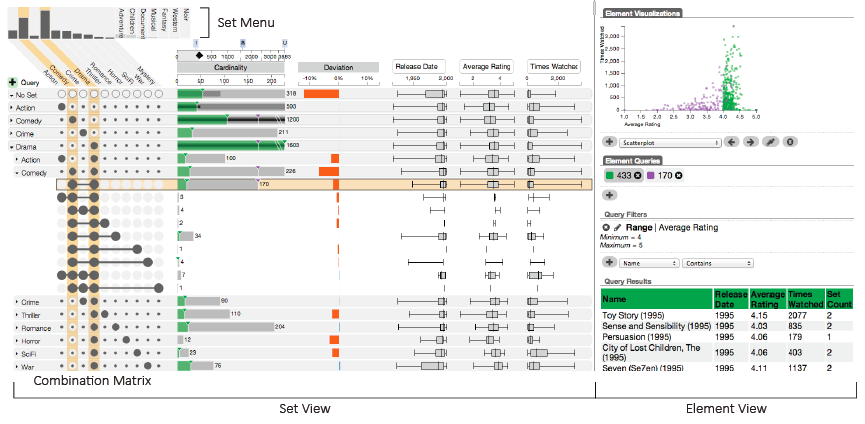
\includegraphics[width=\textwidth]{upsetfig1}
   \caption{UpSet dashboard displaying the relationships amongst movie genres. The left hand side lets the user query the database for a set of movies, listed in the set menu. It then shows how these movies intersect with the other genres of sets. The middle panel shows how many movies are in each intersecting set, and the distribution of select quantitative variables. The right hand panel breaks out the movies in one of these subsets into a scatter plot and a list. This combined visualization tool allows a user to see if quantitative attributes like ratings or times watched can be conditionally dependent on the genre of the movie. This figure comes from UpSet: Visualization of Intersecting Sets \cite{lex_upset_2014}}
   \label{fig:upsetfig}
\end{figure}

The UpSet tool is designed to display a much larger number of set intersections, frequency information about set membership, and the aggregate information of quantitative attributes filtered on sets\cite{lex_upset_2014}. As shown in figure~\ref{fig:upsetfig}, the UpSet tool provides linked set and element views. The set view provides the intersections and their
aggregates, the frequencies of each set and intersection, and the aggregate
statistics of the associated quantitative variables, while the element view shows
selected elements and information about their set membership. The set view yields the distributions of each of the attributes. For example the selected row (in the gray box) are the distributions of each quantitative variable in the comedy set. Every row underneath is the distribution of that quantitative variable restricted to movies in the intersection of the selected sets. For example, the distribution of ratings of movies that are both comedies and dramas. The Upset tool
also facilitates comparison of filtered sets via scatter-plot, which acts as a
visualization of the attributes of the data conditioned on membership in the
filtered set.  The UpSet tool provides a window into conditional dependency because it allows for filtering on sets and then updates the scatter and quantile views; like the scatter matrix, UpSet can isolate a genre or filter on ranges of quantitative variables such that the user can try a variety of approachs to see if there is directionality in the co-occuring events. 
\end{document}


